\documentclass[11pt,letterpaper]{article}
\usepackage[top=1.00in, bottom=1.0in, left=1in, right=1.25in]{geometry}
\usepackage{graphicx}
\usepackage{latexsym,amssymb,epsf}
\usepackage{epstopdf}

\usepackage{sectsty,setspace,natbib}
\usepackage{float}
\usepackage{latexsym}
\usepackage{epsfig}
\usepackage{graphicx}
\usepackage{amsmath}
\usepackage{array}
\usepackage{lineno}
\newcommand{\R}[1]{\label{#1}\linelabel{#1}}
\newcommand{\lr}[1]{line~\lineref{#1}}
\usepackage{gensymb}
\usepackage{xr-hyper}
\externaldocument{phenncc_supp}
% \usepackage{hyperref}

\usepackage{framed}

\linespread{1.1} % was 1.66 for double-spaced 
% \raggedright
\setlength{\parindent}{0.5in}
\pagestyle{empty}

\parskip=5pt
\pagenumbering{arabic}
\pagestyle{plain}
\setlength\parindent{0pt}

\begin{document}
\begin{flushright}
Version dated: \today
\end{flushright}
\bigskip
\noindent Running title: Environmental tracking 
% put in your own RH (running head)
\bigskip
\medskip
\begin{center}
% Insert your title:
\noindent{\Large {\bf How environmental tracking shapes species and communities in \\ stationary and non-stationary systems}}\\
% Other titles: `Environmental tracking: It's more complicated than you think' (we hope) 
% or `Environmental tracking: Is it naive? Or, are we just naive?'
\bigskip
\noindent {\normalsize
E. M. Wolkovich$^{1}$ \& M. J. Donahue$^{2}$ }\\
\noindent {\small \it
$^1$ Forest \& Conservation Sciences, Faculty of Forestry, University of British Columbia, 2424 Main Mall, Vancouver, BC V6T 1Z4 (e.wolkovich@ubc.ca)\\
$^2$ Hawai`i Institute of Marine Biology, University of Hawai`i at M\= anoa, K\=an`eohe, HI 96744 (donahuem@hawaii.edu)}\\
\medskip
\end{center}
\noindent{\bf Corresponding author:} see$^{1}$ above; Ph: 604.827.5246 (no fax).\\

\noindent \emph{Authorship statement:} EMW and MJD both conceived of the paper, performed modeling work and edited the paper, EMW additionally wrote the paper and did the literature review, while MJD additionally wrote the supplementary information on the model.  \\
\noindent \emph{Data statement:} Review, so no new primary data, but data from a comprehensive literature review will be archived in an appropriate public repository and the data DOI will be included at the end of the article. \\
\noindent \emph{Keywords:} community assembly, global change, climate change, phenology, environmental variability\\
\noindent \emph{Article type:} Reviews and Syntheses\\
\noindent \emph{Article information:} Abstract: XXX words; Main text: 6,490; Figures: 4; Boxes: 4 (text in Box 1: 348; Box 2: 500; Box 3: 264, Box 4: 776); 115 references
% main text words (5500 without in-text refs approximately) ... boxes can be a max of 800 words 
\newpage
% \linenumbers % If you want to add need to add \begin{linenomath} and \end{linenomath} around all eqns (and check they still show up)

\linenumbers
\begin{abstract} 
% 198 words
Climate change is reshaping the environments of all species. Predicting responses requires understanding the costs, benefits and constraints of how well species can track environmental change, and how such tracking shapes communities. Growing empirical evidence suggests that environmental tracking---how an organism shifts the timing of key life history events in response to proximate environmental cues---is linked to species performance and is a structuring force of species and communities today. Here, we review current knowledge on tracking both in empirical data and through the lens of ecological theory. We provide a definition of environmental tracking that highlights both why it must be fundamentally related to fitness, and the challenges of defining it empirically. We show how life history theory makes predictions for variation in tracking, and trade-offs with other traits, across species and environments. Finally, we examine how well basic community ecology theory can be extended to test the current paradigm that climate change should favor species with environmental tracking. We to aim provide a framework based on existing ecological theory to understand tracking in stationary and non-stationary systems and, thus, help predict the species- and community-level consequences of climate change.
\end{abstract}
% Finally, we consider how the reality that climate change has widespread effects beyond mean temperature, including shifts in growing season length, variability, and in extreme events, may complicate simple predictions of winners and losers. 
% Limited understanding of organism's phenological cues combined with statistical issues may make many current estimates of variation in tracking less reliable than they appear. Yet these estimates provide the crucial first step to understand variation. 

\newpage
\section{Main text}
Anthropogenic climate change is causing widespread changes in species distributions, with many species shifting in both time and space \citep{IPCC:2014sm}. Reports often focus on species shifting to higher elevations and poleward \citep{Chen2011} and/or shifting their recurring life history events (phenology) earlier as climate warms \citep{Wolkovich:2012n,cohen2018}. These general trends, however, hide high variability across species. A large proportion of species are not shifting at all \citep{Cook:2012pnas}, which has raised concerns about whether these species may be more vulnerable to population declines with continued warming. Such concerns come in part from increasing research that links how well species track climate change---especially through temporal shifts---to shifts in biomass, growth and other metrics related to performance \citep{Cleland:2012}. Tracking climate change may then be a major component to understanding and predicting the indirect effects of climate change, including population declines, with cascading effects on community and ecosystem structure.\R{A1} 

The hypothesis that tracking predicts fitness outcomes with climate change has gained significant traction in the ecological literature focused on global change \citep[e.g.,][]{Cleland:2012} and several areas of ecological theory support it. \R{r1sc1start} Considering tracking as a form of plasticity, evolutionary models predict species that track will be favored in novel environmental conditions. Similarly, some models of community assembly suggest that a warming climate should open up new temporal niche space and favor species that can exploit that space \citep{gotelli1996,wolkovich:2010fee,Zettlemoyer2019}. \R{r1sc2start} Yet not all studies find the purported link \citep[e.g.,][]{block2019}, and there has been comparatively little work to improve predictions by formally connecting tracking to foundational ecological theory. %Thus, a shift toward earlier spring should favor earlier species, especially those that can environmentally track ever-earlier seasons. 

This disconnect could be because most ecological theory today is for stationary systems \citep[e.g.,][]{Sale:1977oq,Chesson:1997dz}. While major arenas of research such as `modern coexistence theory' or population ecology are now built on assumptions of a stochastic environment, they generally still assume stationarity, where the underlying distribution of the environment is unchanged across time \citep[i.e., constant mean and variance,][]{barabas2018}. This assumption is common to much of the theory that underlies ecology, evolution, and myriad other research fields \citep[e.g.,][]{Milly:2008yu,nosenko2013}. 

Climate change upends the assumption of stationarity. By causing increases in temperature, larger pulses of precipitation, increased drought, and more storms \citep{ipcc2013}, climate change has fundamentally shifted major attributes of the environment from stationary to non-stationary regimes (see Fig. \ref{fig:climdat} and Box: Environmental variability \& change). This transition is reshaping ecological systems, and, while new work has aimed to adapt coexistence theory to non-stationary environments \citep{chessonnonstat,volkerass}, there is still little theoretical work on what such a transition may mean for communities and the species within them, despite growing empirical studies.  % Importantly, models based on the theory can help highlight which species `traits,' including those related to how species are matched to and respond to the environment, are favored under different environmental regimes.

Here, we review current knowledge on tracking both in empirical data from the climate change impacts literature and through its related ecological theory. We provide a definition of environmental tracking that highlights why it must be fundamentally related to fitness and the complexity of measuring it in empirical systems. We show how life history theory---specifically drawing on optimal control, bet-hedging and plasticity---make predictions for variation in tracking across species and environments in stationary and non-stationary systems. We then examine how well basic community ecology theory can be extended to test the current paradigm that climate change should favor species with environmental tracking. 

\subsection{Defining environmental tracking}
\R{define1start} While tracking is a commonly used word in the phenology and climate change literature \citep[e.g.,][]{Menzel:2006xn,Cleland:2012,deacy2018}, there are few, if any, definitions of it. Most interpretations of tracking relate to how well an organism matches the timing of a life history event to the ideal timing for that event, what we refer to as `fundamental tracking'. Fundamental tracking thus rests on an assumption that there is a timing (an `ideal timing') that yields maximum fitness, and event timings moving away from this ideal result in reduced fitness \citep[a foundational concept of the trophic mismatch literature,][]{vissergienapp2019}. \R{tmm1}Yet this ideal timing is generally only clear in simplified models or in retrospect, thus species must use environmental cues to attempt to predict and match their event timing to the ideal timing across environments in both space and time (Fig. \ref{fig:defineET}); we call this match between ideal timing and actual timing `cue quality'. Each organism's set of cues forms the biological basis for how a species tracks, but measuring environmental tracking requires two more components.

The first component is the environment's variability---which aspects of the environment vary, how (e.g., temporally each year, spatially at $x$ scale) and how much. If the varying components of the environment are not in the organism's set of cues, then the species may not track this variability. Further, the organism's cues will interact with environmental variability and, thus, under this definition, identical genotypes will have different tracking in different environments.

Second, which aspect(s) of the environment researchers measure will determine `measured environmental tracking'. If researchers know the exact cue (e.g., a thermal threshold) or suite of cues (e.g., a interaction of thermal sums and daylength) and can perfectly measure these in an environment where the cue(s) varies, then an organism will track the environment perfectly. If researchers measure some related attribute (e.g., mean spring temperature in place of thermal sums) or only some of the organism's cues, then the organism will appear to track poorly (i.e., a noisier statistical relationship from poor `measurement quality').  If researchers measure an environmental variable that is not directly related to the cue(s) that the species actually uses, but one correlated with it (e.g., an insect tracks daylength but researchers measure temperature) then they have not measured tracking per our definition.

Accurately measuring environmental tracking thus requires a complete knowledge of an organism's cue(s), the environment's variability and the relationship between the actual cues and measured environmental metrics. Knowing an organism's cues is inherently difficult, generally requiring a suite of experiments, process-based models and in-situ data to show that the model of cues is accurate. Not surprisingly then we lack this for almost all species, coming closest for some model species \citep[e.g., \emph{Arabidopsis thaliana},][]{Kingsolver2007,Wilczek:2009oa}, or species with very simple cues \citep[e.g., coral \emph{Acropora millepora},][]{levy2007} and have some basic information for some other species \citep[e.g., the Great Tit, \emph{Parus major},][]{charm2008}. \R{define1end}

\subsection{Measuring environmental tracking}
\R{newopenmeasure} Attempting to measure environmental tracking and compare variation in it across species, space and time is a rapidly growing area of ecological research \citep[e.g.,][]{Cook:2012pnas,fu2015,thackeray2016,cohen2018}. Multiple meta-analyses now show plants' spring phenology shifts with spring or annual temperatures 4-6 days/$\degree$C on average across species \citep{Richardson:2006qh,Wolkovich:2012n,thackeray2016}, but also highlight high variation across species  \citep{Cook:2012pnas}, even after examining multiple major climate variables \citep{thackeray2016}. Variability across species appears similar when examining consumers tracking their prey \citep[across diverse species tracking over time is 6.1 days/decade but ranges from zero to 15 days/decade, see][]{kharouba2018}. 

All species-rich studies of phenology-climate relationships find high variation, including some species that do not track or track poorly (i.e., high noise surrounding observed statistical relationships). Researchers have worked to link such variation to the underlying cues \citep[e.g.,][]{Cook:2012pnas}, species traits \citep[e.g.,][]{cohen2018} and trophic level \citep[e.g.,][]{thackeray2016}. These approaches hint at the three majors classes of reasons that underlie species that do not appear to track climate (or appear to be poor trackers): (1) species do not track, as perfect environmental tracking may either not be possible or optimal for all species, (2) lack of firm biological understanding of the cues that underlie tracking, and (3) statistical artifacts that make it difficult to measure tracking robustly. 

Increasingly, research has outlined statistical difficulties in measuring tracking. These issues mostly relate to the challenges of observing phenological distributions \citep{steer2019,carter2018}\R{addistribrefs} through anthropogenically defined temporal units (e.g., day or month) in non-stationary systems, and to the complexity of climate data (for further discussion, see Box `Statistical challenges in measuring tracking'). 

Even without statistical issues, translating phenological and climate data into estimates of tracking requires a firm biological understanding of an organism's cues, critical knowledge that researchers rarely have \citep{chmura2019}. Currently, `tracking' is often measured simply as the relationship between the dates of the phenological event and a simple abiotic metric, such as mean monthly temperature (with variation in temperature derived from multiple periods of observation or induced through experiments). Simple environmental metrics, however, are almost always proxies for a more complicated underlying physiology where simple cues---such as warm temperatures---can be modified by other cues, such as photoperiod, drought or light spectra \citep{Bagnall1993,Stinchcombe:2004ec}. Indeed, multiple studies have shown how simple correlations between phenological events and environmental variables can mask complicated relationships \citep{Cook:2012pnas,tansey2017}. % Metrics of tracking are rarely linked to a firm biological understanding of an organism's cues \citep{chmura2019}, which will generally lead to lower estimates of tracking for species with unusual or under-studied cues. 

Modeling multivariate cues well is inherently difficult \citep{chuine2016}, especially since one cue may dominate in many conditions. For example, woody plant leafout responds strongly to warm spring temperatures, but also to cool winter temperatures to prevent leafout in mid-winter warm snaps that occur long before the last frost. Often this cool-temperature effect may be masked by sufficiently cold conditions. With warming from climate change, however, this additional trigger---which appears to vary by site, species and even inter-annual conditions \citep{dennis2003}---may become critical \citep[and potentially lead many phenological models to fail spectacularly in the future as additional cues come into play, see][]{chuine2016}.Tracking in species with longer generation times may be especially complicated, as species may track low frequency climate signals and make investment choices on far longer timescales than species with shorter lifespans \citep{morris2008}. %  In some semi-arid systems, species time growth to pulses of rain, but only when those rain events occur with cooler temperatures that indicate the start of the rainy season, and not a rare summer rainfall event in the middle of months of drought \citep{Wainwright:2012tw,wainwright2013}. 

Researchers are increasingly recognizing the need to consider multiple climate variables, though currently most estimates are based on long-term observational data \citep[e.g.,][]{chmiel2013,simmonds2019}, which can lead to spurious correlations without experiments to test hypothesized cues \citep{chuinearees}. Further, estimates of `tracking' from long-term data that are not linked to mechanistic experiments may sometimes serve as proxies (i.e., environmental variables correlated with one or more actual cue that a species uses) for an organism's environmental tracking, but may not directly connect to an organism's cue(s). 

Limited understanding of organisms' phenological cues combined with statistical issues may make many current estimates of variation in tracking less reliable than they appear, and make robust quantitative analyses across species difficult \citep{brown2016,kharouba2018}. Yet these estimates provide the first step to understand variation. As estimates improve, ecologists will better capture a picture of which species, when, and where, do and do not track. Given the difficulty of measuring environmental tracking currently, clear testable predictions from ecological theory are perhaps most critical to guide research today \citep{Smaldino2016}. \R{endmeasure} % \citep{tourneur2020}

\subsection{Understanding variation in environmental tracking}
A number of research areas in ecology predict variation across species in how well they track the environment. Applying these areas of research to environmental tracking, however, first requires understanding phenological events. In particular, while phenological events are often coded as on/off switches (e.g., a seed does/does not germinate; a coral does/does not spawn), they are almost always defined by investment decisions that are part of a continuous developmental process \citep{inouye2019}. 

\R{whenhow1start}Phenological events can be considered as the outcome of a two-part process that is repeatedly observed over time. At each temporal unit, an event can either happen or not (when - part 1) and, if it happens, the event can vary in size or degree of investment (how much - part 2). This process is generally applied at the level of the individual (but it could potentially apply at lower levels, for example buds on a branch, or potentially higher levels, such as all the offspring from a parent). Across time, it produces an event's distribution. After starting, many events are entrained to continue based on the underlying physiological process: for example, laying eggs within one clutch (here, the first part of the process is whether to lay eggs or not and the second is whether to continue to invest in that process, which would lead to additional eggs, which researchers then observe as number of eggs per temporal unit) or flowering each growing season. In such cases, first events at the individual-level are somewhat unique from the rest of the event's distribution. In all cases, these individual-distributions scale up to the population-level estimates of these events generally used by researchers \citep[see][for discussion of the outcomes of this scaling]{inouye2019}.\R{enddistrib}

Considering the life history events that define part of environmental tracking as a two-part process highlights that tracking is ultimately shaped by resources that species need to grow and reproduce, and circles back to an organism's fundamental tracking. This is perhaps best recognized in the literature on trophic synchrony where there is often focus on how well consumers' environmental tracking matches to the seasonal distributions of their prey \citep{deacy2018,kharouba2018}.\R{tmm2} For example, decades of work has studied how birds (e.g., \emph{Parus major}) time their peak food demands---during their nesting season---to maximum prey (caterpillar) abundance \citep[e.g.,][]{charm2008}. Failure of environmental tracking to match prey year-to-year or over time with long-term warming has been tied to individual-level fitness consequences in some systems \citep{charm2008}, but not all \citep{visser2006}, which may be due to the complexity of mechanisms that influence total fitness \citep{Singer:2010eb,Johansson2012}. Environmental tracking in plants and other lower trophic levels is also about resources. Alpine plant species that emerge in step with snowmelt or temperature are likely responding, at least in part, to light resources for photosynthesis. Light equally appears critical to the sequence of phenology in many temperate forests: with lower-canopy species, and younger (shorter) individuals of higher-canopy species, routinely risking frost damage to leaf out before the canopy closes and access to light becomes severely reduced \citep{Vitasse2013,heberling2019}. These ultimate controllers on tracking---which determine fundamental tracking---are then filtered through the abiotic environmental cues species use to time events (Fig. \ref{fig:defineET}). From here, predicting tracking relates to predicting which cues an organism should use: an optimal control problem.\R{whenhow1end}% In both temperate as well as alpine systems, however, access to critical belowground resources also occurs in the spring---both for available water and for nutrients released with the turnover of seasonal microbial communities \citep{Zak:1990ar,edwards2010N}. Thus, plants' spring phenology in many systems is about careful tracking of nitrogen and other soil resources. As in higher trophic level systems, research has linked how well plants track to performance, with species that track warming tending to grow larger and/or produce more offspring \citep{Cleland:2012}.

\emph{Predicting variation in environmental tracking in stationary systems}\\
\R{constrain1start} An optimal control framing can help predict which cues an organism should have based on a consideration of the costs, benefits, and constraints, in any one organism by environment system \citep{donahue2015}. First, it requires that benefits vary depending on the timing of event; this effect may be stronger in highly seasonal environments. Next, there must be a useful cue---some aspect of the environment that predicts resources or otherwise links to back to the ultimate factors that shape environmental tracking \citep{gremer2016}. Some environments may inherently lack useful predictors, such as desert systems where few early-season variables seem to predict high or consistent rainfall years. 

From here, the exact cue or suite of cue(s) that an organism should have depends on the cost of those cues (e.g., the machinery of monitoring temperature or daylength) and the benefits of a cue (for example, how much tissue is saved by avoiding a coldsnap). Ultimately, the balance of the costs of cue(s) and their benefits should determine what cue(s) a species uses: apparently poor cues may occur for organisms in environments where there is both a low cost and low benefit to the cue(s). Similarly, expensive cues, such as complex multivariate ones, are possible given a high pay-off. Most in-depth studies of species' phenological cues find evidence for complex multivariate ones \citep{chuinearees}. These cues almost always appear adapted to handle unusual---though not completely uncommon---years when the simple cue alone would fail (that is, would trigger growth, reproduction or another life history event at a suboptimal time), suggesting that multivariate cues may provide a large benefit in best coupling the timing of cues to the ultimate controls (i.e., cues that couple environmental tracking strongly to fundamental tracking). 

\R{bh1start}Optimal control highlights that not all species should track, but instead that tracking is based on an optimization of costs and benefits under constraints. In environments where there is no single, predictable optimal time of event, species should bet-hedge - as long as this is allowed under the constraints imposed by an organism's physiology \citep{decasas2015}. In general, species in highly variable environments, or which otherwise face high uncertainty in the timing of investment decisions, should gain a substantial benefit from bet-hedging or employing other approaches that spread out risk given uncertainty \citep{Venable:2007os,donald2013}. Assessing bet-hedging in many systems, however, requires studies of fitness over longer timescales than many current field experiments.\R{bh1end} % bet hedging assumes there is no clear optimum and thus multiple strategies should work and is focused more on how much versus when

Constraints also shape cues and may limit tracking. Fundamental differences in life history impose constraints---for example, the type and amount of loss an organism can sustain each season is limited by its generation time and other attributes related to long-lived lifestages that yield buffered population growth \citep{Chesson:1997dz}. Additionally, constraints may arise if a species cannot closely measure relevant environmental cues \citep{arnold1992,Singer:2010eb}, through unavoidable trade-offs with tracking \citep{Singer:2010eb,Johansson2012}, or through evolutionary pathways. Gene flow from other environments may continually push a population away from its local optimum \citep{lenormand2002}, standing genetic variation limits phenotypic variation and thus can slow the evolution of optimal cues \citep{Franks:2007wd,ghalambor2015}, deeper evolutionary history may produce co-evolved traits making it difficult for selection to act on a single trait axis \citep{Ackerly:2009ly}, or other fundamental evolutionary limits to the rates of trait change and what traits are possible \citep{spandrels}. \R{constrain1end} 

\emph{Predicting variation in environmental tracking in non-stationary systems}\\
Much of life-history theory, including optimal control and bet-hedging, rests on assumptions of stationarity, thus a major open area of research is adapting life history theory to non-stationary environments. Multivariate cues may be especially robust to a non-stationary environment if they provide a tight coupling of cues to fundamental tracking, and that coupling is maintained in the non-stationary environment \citep{dore2018}. But multivariate cues may equally be most vulnerable to failure if non-stationarity decouples the cues from fundamental tracking \citep{bonamour2019}. For example, consider an organism's whose cues evolved based on a correlation between peak prey abundance and daylength---these cues may work well in a stationary environment but fail if warming advances peak prey abundance. Predicting the outcome of non-stationarity thus relies on knowing both the full cue system of an organism, how it relates to fundamental tracking, and how both that cue system and the underlying fundamental model shift with non-stationarity. 

\R{plasticquotestart} Another area of life-history theory, plasticity, may be primed to provide insights on non-stationarity \citep[or `sustained environmental change,' see][]{chevin2010}. Considering phenology as a trait \citep[as we and others do, e.g.,][]{charm2008,nicotra2010,inouye2019}, environmental tracking is one type of plasticity. Researchers could thus more broadly understand environmental tracking through modeling an organism's reaction norms \citep{pigluicci1998,chmura2019} and understanding how cues and suites of cues---across environments---determine how fundamentally plastic an organism may be in its tracking. For example, multivariate cues should yield higher plasticity in this framework. From here, models of the role of plasticity in novel environments provide an important bridge to understanding the outcomes of non-stationarity, generally predicting non-stationarity should favor highly plastic species. This outcome, however, assumes there are no costs related to plasticity \citep{Ghalambor2007,tufto2015}. If there are costs associated with plasticity (here, directly akin to costs associated with tracking), then species may evolve lower tracking, because it should trade-off with other traits \citep{auld2010}. \R{plasticquoteend}

\subsection{Tracking in multi-species environments} 
\R{sectionmutisppstart} Plasticity theory---in contrast to much of the life-history theory discussed above (where other species are, at best, filtered into models as an aspect of the environment)---shows how critical a multi-species perspective is to understanding environmental tracking \citep{metcalf2015}. In this light, tracking cannot be considered as a singular trait, but must be evaluated as part of a trait syndrome \citep[or mosaic of traits,][]{Ghalambor2007} and selection in multi-species environments should produce communities of species where tracking trades-off with other traits. 

\R{traittradeoffstart}As tracking often relates to the timing of a resource pulse, traits related to resource acquisition are likely contenders for a trade-off. Species with traits that make them poor resource competitors may need to track the environment closely to take advantage of transient periods of available resources, but will risk tissue loss to harsh environmental conditions more prevalent early in the season (e.g., frost or snow). In contrast, species with traits that make them superior resource competitors may perform well even if they track environments less closely, because their resource acquisition is not strongly constrained by competitors. Examples include under-canopy species leafing out earlier to gain access to light \citep{heberling2019} or species with shallow roots starting growth sooner in an alpine meadow system, while species with deeper roots begin growth later \citep{Zhu2016BioLetters}. In such cases, tracking is akin to a competition-colonization trade-off \citep{Amarasekare:2003tq}, where species that track well gain priority access to resources and, thus, may co-exist with superior competitors. Research to date supports this, with several studies linking higher tracking to traits associated with being poor competitors \citep{Dorji2013,lasky2016,Zhu2016BioLetters}. Further, many studies have found a correlation between higher tracking and `earlyness' each season, which has been linked to resource acquisition traits associated with lower competitive abilities \citep[][see Box `Trait trade-offs with tracking']{wolkovich2014aob}. \R{traittradeoffend} 

Understanding these trade-offs is clearly critical, but understanding the short-term dynamics of a changing environment with plastic species is additionally important. Most theory predicts the outcome of a new environment, but non-stationarity in the climate today means understanding the trajectory to that outcome may be most relevant. For example, models show how plasticity may limit standing variation and thus reduce fitness in novel environments \citep{Ghalambor2007,fox2019}. Whether such findings extend to systems transitioning from stationary to non-stationary will likely depend on how non-stationarity affects the rate of adaptation \citep{chevin2010}. Efforts to model expected outcomes given climate projections and current understanding of plasticity and genetic variation underlying event timing in some organisms provide the empirical start to this \citep[e.g.,][]{fournier2016}, but more eco-evolutionary models that bridge this gap may prove especially useful. \R{endplastic}

\emph{Including tracking in multi-species community assembly models} \\
\R{startmodels}Predicting how tracking may determine which species are effectively winners and losers with climate change requires integrating non-stationary environments into models of community assembly. Recent advances in coexistence models, sometimes called `modern coexistence theory,' recognize that both mechanisms independent of fluctuations in the environment (e.g., R* and other classical niche differences) and mechanisms dependent on fluctuations in the environment (relative non-linearity and storage effect) can lead to coexistence \citep{Chesson:1997dz,Chesson:2000vd}. These models, which underlie much of current community ecology research \citep{Mayfield:2010fe,barabas2018,ellner2019}, provide a framework to begin to model environmental tracking and non-stationarity. 

How the environment is defined in most community models falls into two broad categories. In some models the environment is expressed as variation in parameters related to species. For example, in some lottery models the environment appears, effectively, as variation in birth and death rates. \R{S2start}Building a changing environment into such models thus requires knowing how environmental shifts filter through to species-level parameters \citep{Tuljapurkar2009}. For example, \citet{volkerass} added the temporal environment to competition models by defining interaction strength as dependent on the temporal distance between species. This is somewhat similar to models that include the the environment effectively through different levels of asynchrony \citep[e.g.,][]{Nakazawa2012,revilla2014}. \R{S2end}In other models, the environment is more specifically defined. Many of these models define the environment as a resource (e.g., many seed germination models that begin with a resource pulse each year), and thus generally model something close to fundamental tracking. Building a changing environment into these models requires knowing how the environment is changing.

Models that explicitly include the environment provide a major opportunity to predict how environmental tracking and non-stationarity determine future communities (see Box: `Adding tracking and non-stationarity to a common coexistence model'). Yet most current models generally examine the environment from only one of two relevant angles: they represent the environment as used for species' cues (e.g., many models of plasticity) or they represent the environment as directly affecting fitness (e.g., the storage effect model). Combining these two angles may be especially critical to understanding the costs and benefits of tracking in non-stationary environments. \R{modelcosts1} 

% Lottery model: Birth and death rates vary ... collapses to single ratio (that's the environment) ... many general models are like this, they just vary a parameter and assume it is varying in response to the environment. Whatever parameter you allow to vary is how you allow the environment to filter through. (Side note: Tulja Purqur may have worked on how environment filters through to many species parameters in the model.)

\R{whenhow2start}Layered onto the different angles that different models take on the environment is how species responses to the environment are defined. In general, species responses to the (resource) environment can be broadly grouped into models that explicitly define when species start an event (e.g., spawning or germination) in response to the environment versus those that model the magnitude (e.g., the number of propagules or seeds) of response to the environment. Models that explicitly model when a species starts an event are often focused on situations where order of arrival is critical to predicting coexistence outcomes. For example, models of priority effects through niche pre-emption highlight the advantage tracking may provide when it allows species to be early (and when there is no cost to being too early): early arrivals receive a head-start advantage, by gaining priority access to resources (the environment) they can draw down the resources available to later arrivals \citep{fukami2015}. Such models predict the early-arriving species to out-compete other species, unless the order of arrival varies by year or there are trade-offs with other species' traits (see Fig. \ref{fig:conceptmodels}).
% If one species is always early there has to be a trade-off. [Each year every species has a similar advantage and it's the same advantage every year, you could predict it with one year; in the other model the density effects are more variable by year -- you need inter-annual variation to predict the outcome. ]

 % Species that track in this model could be considered those that arrive earliest, however, priority effects generally require species that are highly similar to one another and thus models of priority effects do not predict variation in tracking across species, and further would not predict trade-offs between tracking and other traits \citep{fukami2015}. Trade-offs, however, are predicted from competition/colonization models: if species that track well are akin to species with high-dispersal, trackers may coexist by gaining early access to resources and reproducing before the later arrival of superior competitors. 
Other models canalize species' responses to the environment into production and investment. For example, most models of inter-annual competition (much of `modern coexistence theory') fall into this camp. Species produce (via offspring, tissue etc.) differentially depending on the environment each year and outcomes are mediated through density. While these models superficially may seem disconnected from timing, they critically highlight how phenology relates to production and, thus, investment across years. Further, they almost always model the environment as a distribution (see Fig. \ref{fig:conceptmodels}), which provides the opportunity for the environment to alter the competitive environment each year and, thus, structure coexistence. % These models can be used to investigate tracking by modeling the match of a species to its environment that varies from year to year where in some years one species has the advantage and in other years the other species will. 

\R{whenhownewmod} A model where species vary both when they start an event and how much they produce dependent on the environment would capture the important attributes of tracking---combining head-start advantages from being early with production variation based on the fitness of the environment. To our knowledge, however, most models approach these questions separately, though models of bet-hedging come closest \citep{Gourbiere2009,tufto2015}. A model that explicitly models the linked decisions of when to time an event and how much to offspring/tissue to produce during the event could provide fundamental insights on the relative importance of each aspect of this process. Such a model could be adapted to address multiple questions of environmental tracking, including how these decisions (`when' and `how much') may trade-off and which other traits may be most strongly linked to tracking, as well as explicitly modeling the costs and benefits of tracking in stationary systems -- \R{modelcosts2}a critical precursor to extending it to non-stationary systems. \R{whenhow2end}

Extending models to non-stationary systems is crucial to testing how environmental tracking relates to species persistence with climate change, and research has already begun to tackle this non-trivial challenge \citep{chessonnonstat,legault2019,volkerass}. Most work to date, however, focuses on conclusions from stationary or non-stationary systems. Thus, the transition between stationary and non-stationary is often ignored, yet we expect it may be most critical. Communities formed in stationary environment periods (or periods with environments lower non-stationarity) are effectively filtered and assembled by that environmental regime and thus produce the baseline of variation and assembly dynamics for a shifting environment. While analytical solutions for systems transitioning from stationary to non-stationary may take time to develop \citep{chessonnonstat}, simulation work can provide an immediate intuition and framework to address this challenge (see Box: Adding tracking and non-stationarity to a common coexistence model). \R{sectionmutisppend}

\subsection{Future directions}

Growing empirical research highlights that environmental tracking is linked to species performance and, thus, may be critical to understanding the forces that assemble communities and determine species persistence---especially as anthropogenic climate change is reshaping the environment of all species. Ecological theory, including from areas of optimal control, plasticity, coexistence, and community assembly, is clearly primed for understanding how a variable environment can shape the formation and persistence of species and communities. To understand what advances in theory may be most useful for making predictions in the Anthropocene, we need more focus on understanding the attributes of an environment shaped strongly by humans. In turn, to test theory we need more robust estimates of environmental tracking and how it fits within a mosaic of other correlated traits. To this aim, we review several major areas of research that we believe could most rapidly unite empirical and theoretical research in environmental tracking to advance the field.\\ % Including non-stationarity in ecological theory is non-trivial \citep{chessonnonstat,legault2019}, but is the current environment in which all observational ecology occurs.

\emph{How is an organism's environment changing?} \\ 
Currently, much research has focused on one major shift in the climate system (earlier growing seasons), but research on multivariate environmental shifts is growing and will be critical to understanding how climate change affects an organism's whole environment. Ecologists can guide these efforts by identifying environmental shifts that are often linked (e.g., warming temperatures may drive earlier seasons and higher evaporative loss of some resources such as water). Researchers can also aim to more consistently and fully characterize the environmental distributions of their systems that appear to drive species performance and interactions: the environment of the years of study should be clearly reported and compared against long-term and recent climate for each system. 

More interdisciplinary research with climate science could also speed a fuller understanding of what shifts are and are not expected with climate change, and what climate variables are inherently correlated. Such correlations make estimating cues and other biological parameters from long-term data especially precarious \citep{tansey2017}. But these correlations are equally critical in considering how species may view their environment and whether environmental change will couple or uncouple links between proximate cues and fundamental tracking \citep{bonamour2019}. \\

\emph{Understanding and measuring `tracking'} \\
\R{understandquotestart}Understanding how the environment is changing represents just one step towards robust measures of environmental tracking. Shifting environmental regimes must then be filtered through species cues. As robust estimates of these cues are currently available for few species, we suggest several major improvements on current methods to help interpret current trends and make comparisons more feasible. 

Studies should clarify their definition of tracking, how the environment is defined and how well, or not, the underlying cue system is understood for study species. Currently, many studies examine fundamental and environmental tracking at once \citep[e.g.,][]{yang2020},\R{yang2020} which is clearly helpful in advancing the field. However, the more researchers can clarify when and how they are addressing fundamental tracking versus environmental tracking, the more easily we can compare results across studies. Next, and relatedly, studies should define their environment: are they considering primarily the abiotic environment or measuring an environment fundamentally shaped by other species? This difference connects to fundamental versus realized niches and whether systems are primarily top-down (resources and the environment may be strongly shaped by other species) or bottom-up controlled. Finally, all researchers working on environmental tracking need to embrace their inner-physiologist, or collaborate with one. For many species, there is often a related species (albeit, sometimes distantly) whose cue system has been studied. Thus, researchers should draw on the literature of their study species' close relatives to bracket which environmental variables may represent environmental tracking and which may be proxies and to highlight uncertainty. We expect progress will come from a balance between measures of fundamental tracking, estimating an organism's system of cues, and measuring environmental tracking. Clear statements of what is and is not known and measured will help. 

Embrace the sometimes contradictory pulls of conducting experiments to identify mechanistic cues and the multivariate climate of the real world. Clearly, we need more experiments to identify which specific aspects of the environment different species cue to and how these cues are filtered by their actual environmental regime \citep[as outlined above and see][]{chmura2019}. Suites of experiments, which build from identifying cues to understanding how they act when correlated, are a major gap for most organisms. \R{understandquoteend}

Build a model of your species' cues and interrogate it. As research progresses in trying to estimate environmental tracking, greater progress will come from fuller and more diverse interrogations of current (and future) models. Define the framework under which you expect your cue system developed or works (e.g., bet-hedging) then test how well it works, and where it fails \citep[see][for an example]{johanOCR}. Model interrogation can also use realistic environmental regimes to provide field predictions \citep{Wilczek:2010ad,Wilczek:2009oa} or predict future species and communities. One example of this comes from in silica resurrection experiments of model organisms where future environmental regimes included a mix of regular climate projections and projections modified to test and advance understanding of environmental tracking for the study species \citep[e.g., warmer winter and altered photoperiod scenarios in][]{fournier2016}.\\

\emph{What major traits trade-off with tracking?} \\ 
\R{fdtradeoffsstart}Basic theory of plasticity and competition suggest that environmental tracking must trade-off with other traits to allow multi-species communities. Yet to date empirical work has mainly documented tracking, linked it to performance, or focused on how it varies between native and non-native species \citep{Willis:2010al,wolkovichAmBot2013,Zettlemoyer2019}. Such work lays the groundwork that environmental tracking is important, but future empirical research should address how this trait co-occurs with other traits. Research has highlighted some traits that co-vary with tracking \citep[e.g.,][]{kharouba2014,lasky2016,Zhu2016BioLetters}, but to tie this empirical work to models requires more research on traits that link clearly to theory, and a fuller understanding of how tracking and other traits jointly contribute to performance under varying environments. 

Traits that link to resource competition, as we focus on here \citep[as others have as well, see][]{volkerass}, may be especially fruitful for greater research, but should not be the only ones considered. For example, traits related to predator tolerance or avoidance may also play a role, but have been effectively unstudied.  As empirical research in this area grows, models can aid progress in understanding the outcomes of these trade-offs for community assembly. \R{fdtradeoffsend}\\ 

\emph{Developing new models for tracking in stationary to non-stationary systems} \\ 
As outlined above many areas of ecological and evolutionary modeling contribute to our understanding of environmental tracking. But most are limited in various ways. Community ecology models generally bifurcate in modeling differences in timing versus production amounts across species, thus studies of whether these models lead to similar or different conclusions would help predict community outcomes and advance our understanding of trade-offs. As outlined above, understanding tracking likely requires models that combine effects. This includes models that combine effects of variation in timing and production amounts and models that include environment as impacting species' cues, as well as species' fitness. Such models would explicitly allow the potential costs and benefits of tracking \R{modelcosts3} depending on how closely environmental tracking matches fundamental tracking.

New models will also need to examine how relaxing assumptions of closed communities (i.e., without dispersal or evolution) alter predictions. In practice, dispersal of species or individuals with traits that make them better matched to the non-stationary environment would lead to new communities that may persist or be continually re-assembled as long as the environment remains non-stationary. Indeed, this logic underlies the argument that invasive species may be superior trackers benefiting from how climate change has altered growing seasons \citep{Willis:2010al,wolkovich:2010fee}. Evolution equally could alter predictions by allowing species traits to evolve in step with environmental change. Long-term population \citep[e.g.,][]{colautti2017} and resurrection studies \citep{wilczek2014,yousey2018}, as well as field experiments \citep{colautti2017,arab2019}, have repeatedly shown species can shift to earlier flowering times, higher thermal tolerances or related genetically-controlled traits that confer higher fitness in warmer climates. Yet these studies also highlight that responses can be lagged \citep[e.g.,][]{wilczek2014}, associated with reduced population viability \citep[e.g.,][]{colautti2017}, or other factors that may constrain adaptive responses. \R{constrain2}
% In practice, communities may lose species but also gain new species through dispersal, allowing communities to potentially adjust to new trade-offs as the environment shifts. In addition, evolution may allow some species to stay in communities they would otherwise have been lost from. 
% But with non-stationarity this axis is constantly shifting---so continual community change via species loss, gain and reshaped species via evolution may be the expectation, until the environment shifts back to stationarity.

\subsection{Stationarity in the future}

\R{nsfutstart} While most environments today are climatically non-stationary and have been for decades, the climate will return to a more stationarity form in the future. There are many possible pathways to climatic stabilization, but almost all require first the stabilization of greenhouse gases---the subject of much policy and political debate. Once greenhouse gas emissions stabilize climate will not quickly snap back to a new stationary phase. Instead systems will slowly approach a new climatic stationarity depending on how they are effected by the earth's multiple thermal reservoirs, and, in turn, how quickly those reservoirs stabilize. The timescale of this approach is generally expected to be on the scale of centuries, but could be much longer in certain oceanic systems \citep{ipcc2013ch12}. Thus, ecologists are---and will remain for the foreseeable future---in a research area structured by climatic non-stationarity. 

As paleobiologists and evolutionary biologists often point out, climatic nonstationarity is a common part of the earth's history \citep{Jansson:2002nz}---even if stationary periods---be they cold or warm (glacial and interglacial periods)---are more common. Indeed, while much of this work has examined how species survive for millions of years given large oscillations in climate \citep{provan2008}, the periods that provide the most dramatic community reshuffling are periods shifting from stationary to non-stationary climate regimes \citep{vrba1980,vrba1985}. Such stories of the past are now fundamentally happening today, and ecology is challenged to understand how transitions between stationary and non-stationary environments are reshaping the species and communities we have today and will in our warmer future. \R{nsfutend}

\section{Acknowledgments}
We thank I. Breckheimer, D. Buonaiuto, E. Cleland, J. Davies, G. Legault and two anonymous reviewers for helpful comments that improved the manuscript and the NSERC Discovery Award (RGPIN-05038 to EMW) and Canada Research Chair in Temporal Ecology (EMW) programs that provided funding. 

% Chapter 12 of IPCC WG1 "Long-term Climate Change: Projections, commitments and irreversibility" (Section 12.5: Climate Change Beyond 2100, Commitment, Stabilization and Irreversibility)

% Note to self: environmental tracking seems used by spatial folks ...
   % https://www.nature.com/articles/srep36265
% But! The temporal autocorrelation folks use it too ... this is mainly one-site population work I think and pretty damn similar to our use!
   % https://royalsocietypublishing.org/doi/10.1098/rspb.2011.0487 (2011)
   % https://link.springer.com/article/10.1007/s12080-015-0276-6 (2016)
   % https://besjournals.onlinelibrary.wiley.com/doi/full/10.1111/1365-2745.12077 (2013) 
% And this annual review has a whole section (no definition though that I saw):
   % https://www.annualreviews.org/doi/full/10.1146/annurev.ecolsys.35.120202.110110 ... about fossil 'The principal cause for these patterns appears to be species-, and perhaps clade-level, environmental fidelity that results in long-term tracking of physical conditions. ... biotas do appear to track climates, but such tracking is certainly influenced by geographic and physicochemical barriers' 
% So I say it is all the same thing! And we focus here on the temporal aspect .... give nod to space at the end of ms maybe?


%%
%%
%%
%%
%%

% We believe robust comparisons of tracking metrics require more efforts to estimate the full suite of cues species use, or at least bracket its uncertainty, then connect it to environmental variability and what aspects of the environment the researchers have measured. Yet estimates likely capture important realities of environmental tracking. 

\newpage
\section{Boxes}

\subsection{Box: Environmental variability \& change} % 348 words
Decades of ecological research highlight how temporally variable environments shape species and their communities at multiple scales \citep{Sale:1977oq,Chesson:1997dz}.  In seasonal landscapes, the environment limits periods for growth each year (e.g., by temperature or drought); within-year variability in the environment (e.g., daily, hourly or finer resolution temperatures or rainfall amounts) compounds into inter-annual variability that shapes the distribution of the start and end of growing seasons. For long stretches of history this variability has been effectively stationary; that is, the underlying probability distribution that describes the start (or end) of the season (e.g., the date of the last major frost) does not change, even though the date may be dramatically different from one year to the  next. % The shape of this underlying distribution varies across systems and in how it is measured---for example, the total amount of rainfall across years in semi-arid systems is often highly skewed (rare high rainfall years, with many more below-average rainfall years) compared to the more normal (Gaussian) distribution of the thermal sum of temperate growing seasons. 
% In seasonal landscapes, periods for growth each year are limited (e.g., by temperature or drought), and species must manage within-year variability by timing when to grow and when to reproduce \citep{donohue2002}. 

In other time periods, variability has been non-stationary in one or multiple dimensions. For example, climate in the northern hemisphere includes long warming and then cooling periods (i.e., increasing then decreasing means of the probability distribution) at the start of the Holocene, when the earth was coming out of the last glacial maximum. Anthropogenic climate change is a similar non-stationary process, with warming evident around the globe and knock-on effects for other climate metrics, such as heat extremes and the size of precipitation events. % While only several decades ago, ecology was focused strongly on stochasticity in stationary systems \citep[e.g.,][]{Ripa1996,Kaitala1997}, climate change has shifted the focus to understanding stochasticity in a non-stationary framework \citep[e.g.,][]{cazwavelets,ehrlen2016,legault2019}.

Understanding non-stationarity in ecological systems requires first identifying which aspects of the environment have shifted---and how they have shifted with respect to one another---as the underlying  distributions transition from stationary to non-stationary (Fig. \ref{fig:climdat}). For example, with climate change, warming has increased mean temperatures over time, with minimum temperatures generally increasing more than maximum---this results in an underlying distribution for daily temperature where the mean is increasing through time while the within-day variance is decreasing \citep{ipcc2013,screen2014}. \R{nsstart} Understanding the impacts of climate change further requires recognizing that most systems can be considered stationary or non-stationary depending on the timescale and period of study. Thus, predicting the consequences of current non-stationarity in ecological systems benefits from identifying the type and scale of non-stationarity, relative to long-term trends. \R{nsend} 

\subsection{Box: Statistical challenges in measuring tracking} % 500 words ... Analyses of long-term observational data are also the most at risk of interpreting statistical bias or artifacts as biology.
A potentially widespread reason for observations of species that do not track is statistical bias and artifacts, including non-stationarity in units and unrecognized low power. All of these can be addressed given improved statistical approaches \citep[e.g.,][]{gienapp2005,pearse2017}, though such approaches may uncomfortably highlight how uncertain many current estimates are \citep{brown2016}. Non-stationarity in units comes in many forms---estimates of mean days shifted per decade (i.e., days/decade, a common metric summarizing observed shifts in phenology over time in long-term datasets) depend strongly on the climate of the decade(s) studied, which is not consistent in many systems \citep{Ault2011,McCabe2012}. Estimates based on a relevant climate variable can sometimes ameliorate this problem, but may be equally vulnerable to non-stationarity in units \citep[e.g.,][]{Sagarin:2001fu}. For example, processes that depend on thermal sums reported as days/$\degree$C will generally appear to decline with warming, as the thermal sum of an average day has increased in most regions with climate change. Relatedly, estimates of long-term change using simple linear regression are influenced by the climate at the start of the time-series (with greater changes seen from time-series that started in unusually cold decades, such as the 1950s for much of North America). Impacts of start-years for long-term time-series can be muted by applying change-point or hinge models \citep[e.g.,][]{kharouba2018}, while metrics that move away from calendar units (e.g., day) can help address non-stationarity in units. 

Low power is widespread in ecology, where even `long' time-series may be far too short for robust analyses \citep{bolmgren2013,kharouba2018}. Authors should be especially cautious if they find only large effects appear significant \citep[e.g.,][]{CaraDonna2014}, which is a well-known statistical bias associated with p-values \citep{loken2017}. Additionally, effect sizes that are higher when climate variability is higher (for example, in temperate habitats temperature is highly variable in the spring and autumn compared to summer) may be more related to variation in statistical power than to biology (periods with higher variation yield greater variation in the predictor variable, and thus higher power). Mixed models can help better leverage understanding by pooling information across species, and often better capture uncertainty \citep{pearse2017}. We suggest mixed models should be used more widely alongside randomization and/or data-simulation approaches \citep[e.g.,][]{bolmgren2013,kharouba2018} to better estimate and communicate uncertainty in studies. And researchers should identify what results bias may produce. For example, growing evidence suggests a potential fundamental trade-off where early species track and possess a suite of traits to related to faster growth and shorter lifespans, while later species track less and possess traits related to slower growth and longer lifespans---these later species may bet-hedge more given their longer investment window. \R{bh3}This, however, could equally be an artifact where early species use simpler cues, and, thus, their tracking is measured more accurately given current methods.

\subsection{Box: Trait trade-offs with tracking} % 264 words
% Supp figure is still not showing -- comes up with ?? in Figure reference.
Research on phenological tracking and traits has increased greatly in recent years, with a major uptick in studies after 2010 (see SI Fig. \ref{fig:papertrends}). Most papers examining tracking and other traits across species have focused on plants (20/30), followed by birds and Lepidoptera (both 4/30), plankton and aphids (both 1/30). The most studied trait was how early or late a phenophase occurred (e.g., date of flowering of start of migration for a species, termed `earlyness' by some authors), with earlier species tending to track more \citep[studies included both birds and Lepidotera,][]{Diamond:2011nx,Ishioka2013,kharouba2014,jing2016,du2017}. While this is an important link, it is vulnerable to statistical challenges (see Box `Statistical challenges in measuring tracking'). Few studies examined whether tracking correlates with resource acquisition traits; those that did generally found species with higher tracking also had traits associated with lower competitive abilities under low resources \citep[e.g., being shallower or lacking a taproot rooted][]{Dorji2013,lasky2016,Zhu2016BioLetters}. These species were often also early \citep[e.g.,][]{Dorji2013,Zhu2016BioLetters}, suggesting tracking may relate to a syndrome of traits that allow species to be rapid colonizers each season, but poor competitors for resources. Indeed, previous work has documented that species with earlier phenophases tend to have resource acquisition traits associated with lower competitive abilities \citep[e.g., they tend to be of lower height, have shallower roots, narrower diameter vessels, thinner leaves, and grow faster, reviewed in][]{wolkovich2014aob}. % See \cite{kimball2012,huang2016} as contrast....
% need to add Jing2016 to "studies included both birds and Lepidotera"

\subsection{Box: Adding tracking and non-stationarity to a common coexistence model} % 776/800 words now
To understand the role of environmental tracking by species in variable environments we use a simple model that allows within- and between-year dynamics to contribute to coexistence. As the model is akin to many commonly used seed germination models \citep{Chesson:2004eo}, we follow a similar terminology for ease; however the basic structure of our model could apply to other systems with one dominant (non-renewing) \R{nonrenew} pulse of a limiting resource each season (e.g., water from rain or snowpack), or a multivariate resource pulse that acts effectively as one resource (e.g., nitrogen and light drawn down together over the season). In this model the environment is included between-years via variable germination, and within-years the environment is explicitly included as a resource pulse at the start of the season. We adjust the biological start time of species ($\tau_i$ for species $i$) to also allow species to respond to the environment dynamically through what we refer to as tracking. Here, tracking effectively moves a species intrinsic start time closer to the environmental start time in that year, resulting in a higher germination fraction (see SI for complete description and equations).

Species can co-occur via equalizing mechanisms, but they require stabilizing mechanisms to coexist. Species that is, cannot coexist given only variation in tracking---coexistence requires variation in another trait axis. As theory and empirical work suggest this trade-off may involve traits related closely to resource competition, we varied species' $R^*$. With variation in tracking and in $R^*$ species can persist together as long as those species with a temporal niche advantage are also the inferior competitors (Fig. \ref{fig:modelfig}). That is, species that can draw resources down to a lower level and are thus the superior within-season resource competitors (lower $R^*$) can persist with species with that are inferior competitors but have realized biological start times closer to the environmental start time---a finding inline with currently observed empirical trade-offs (see Box `Trait trade-offs with tracking'). These trade-offs, however, are all environmentally dependent. They hold only so long as the environment is stationary. 

We examined how trade-offs may be transformed by a non-stationary environment, by transitioning a stationary environment---in which two-species communities had persisted for 500 years---to non-stationary, via an earlier start of season (earlier timing of the resource pulse, $\tau_p$, Fig. \ref{fig:modelfig}; see SI for more details). By changing a fundamental niche axis (the distribution of the environment, an axis along which these communities were structured), we shifted one major part of the trade-off: the new non-stationary environment favored an earlier start time than the previous stationary environment. This, in turn, reshaped our two-species communities, which depended on this trade-off for persistence. 

While the non-stationary environment favored higher trackers (who in turn drove the extinction of species with lower tracking values from many two-species communities) some two-species communities persisted (257 out of 1698 two-species communities persisting after end of stationary, or 15.1\%, Fig. \ref{fig:modelfig}). These two-species communities persisted because the same fundamental trade-off between biological start time and within-season competitive ability, while narrowed, was not fully lost. Taken together, these simple simulations show how non-stationarity can drive local species extinction and reshape the underlying assembly mechanisms of communities.

Our simulations support growing work that tracking should not be considered alone \citep{Diamond:2011nx,Dorji2013,Ishioka2013,kharouba2014,du2017}, but may be part of a larger trait syndrome. Indeed, this model trivially show that multi-species communities cannot form given only variation in the temporal niche---a trade-off is required. Our results thus support empirical work showing a trade-off where trackers are also inferior resource competitors \citep{lasky2016,Zhu2016BioLetters}---we show this must be the case for multi-species persistence; otherwise, the species best matched to the environment would drive the other extinct.

Finally, our results highlight that non-stationarity may reshape the balance of equalizing versus stabilizing mechanisms. As environments shifted from stationarity to non-stationarity, species that co-occured via equalizing mechanisms persisted longer. While the outcome that equalized species will be more similarly affected by environmental shifts is rather obvious, it has several important implications. First, it may make identifying which traits climate change promotes through stabilizing mechanisms more difficult. Second, it suggests climate change---or other factors that cause an environment to shift from stationary to non-stationary---may cause a fundamental shift away from assembly via stabilizing mechanisms. % Thus understanding the prevalence of stabilizing versus equalizing mechanisms \citep[which ecology has worked on for many decades,][]{Caswell:1976np,Chesson:2000vd} becomes critical for understanding the implications of transitions to non-stationary environments. 


%=======================================================================
% Figures
%=======================================================================
\clearpage
\section{Figures}

\begin{figure}[h!]
\centering
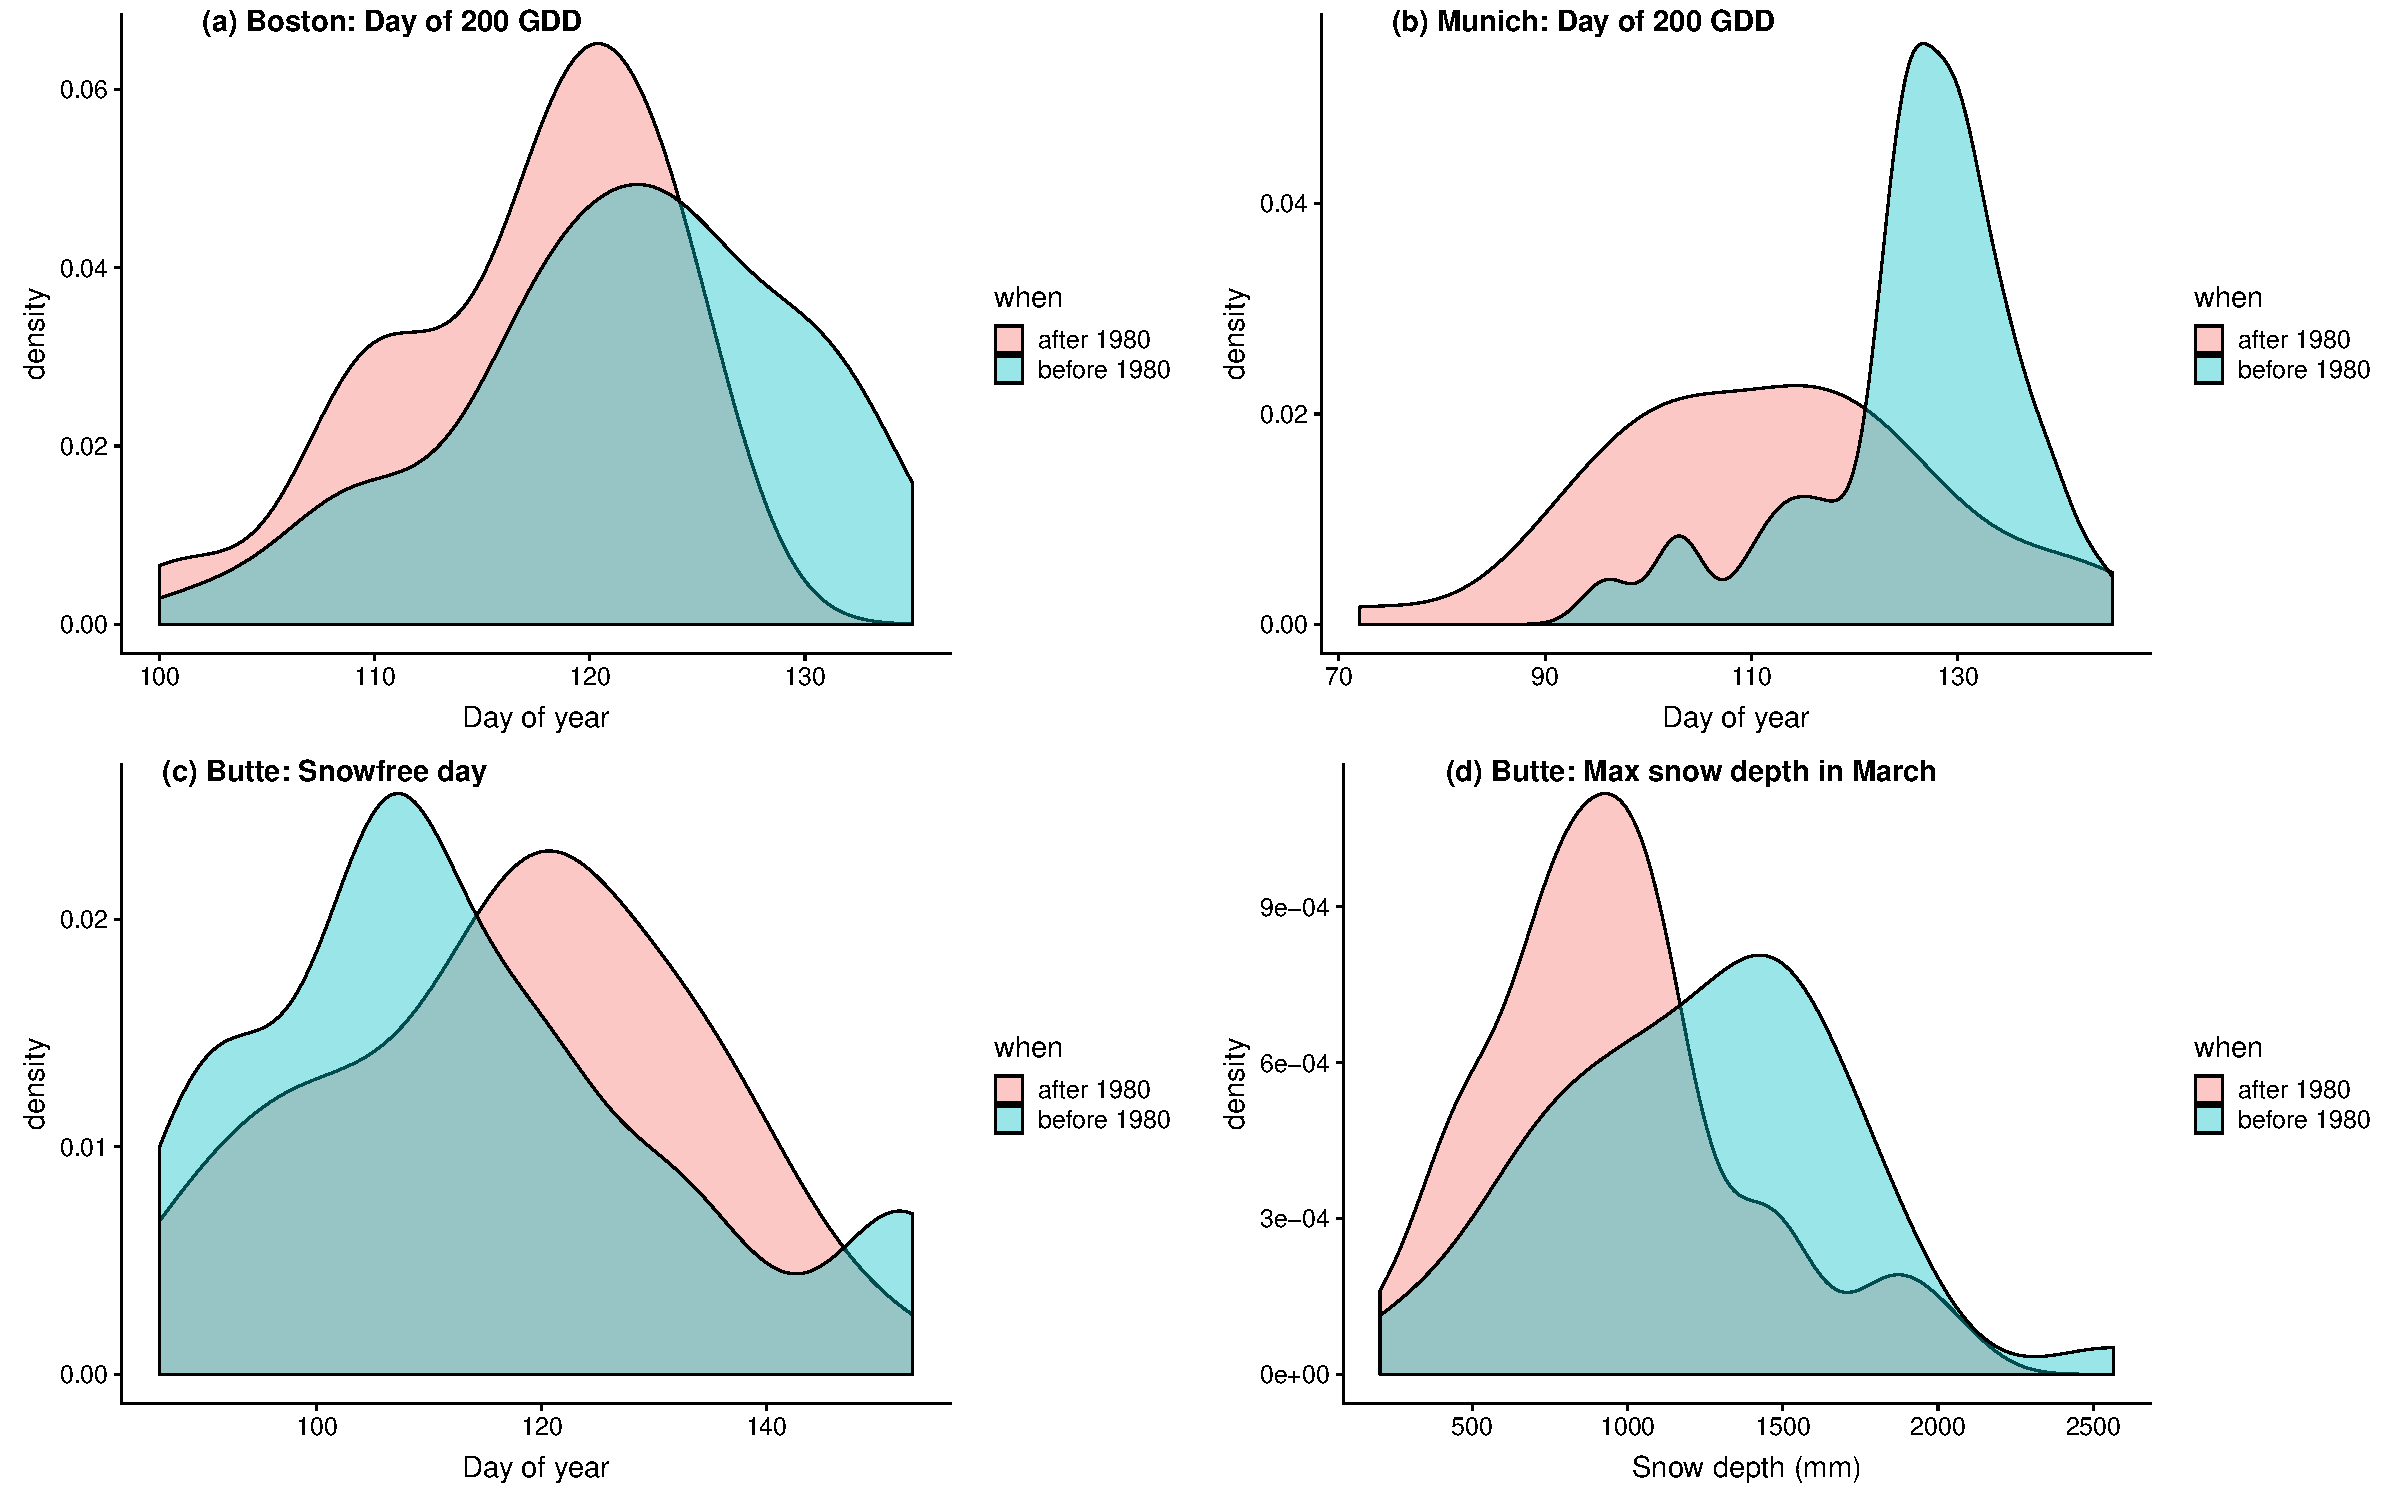
\includegraphics[width=1\textwidth]{..//..//..//R/graphs/otherdat/climdata.pdf}
\caption{Examples of non-stationarity in climate variables linked to environmental tracking: shifts before and after 1980 (a major change-point in climate for many regions) in several metrics related to the start of growing seasons (a-c) or resource pulse connected to growing season length (d). Density plots of day of 200 growing degree day units (a metric of thermal sum, here based on 0 degree base temperature using daily minima in $\degree$C) in Boston, MA, USA (a), and Munich, Germany (b), first snowfree day (followed by at least 9 snowfree days) in Crested Butte, CO, USA (c) and maximum snowdepth (mm) in March (often the month before the first snowfree day) in Crested Butte, CO, USA (d). Note that (c) and (d) are likely related, with lower snowpacks leading to an earlier first snowfree day. We selected sites that have been studied for plant phenological data and included at least 80 years of daily climate data from a Global Historical Climatology Network site; we subsetted data so that there were 40 years before and after 1980 for all sites.} %  (downloaded from \href{https://climexp.knmi.nl/})
 \label{fig:climdat}
\end{figure}

\begin{figure}[h!]
\centering
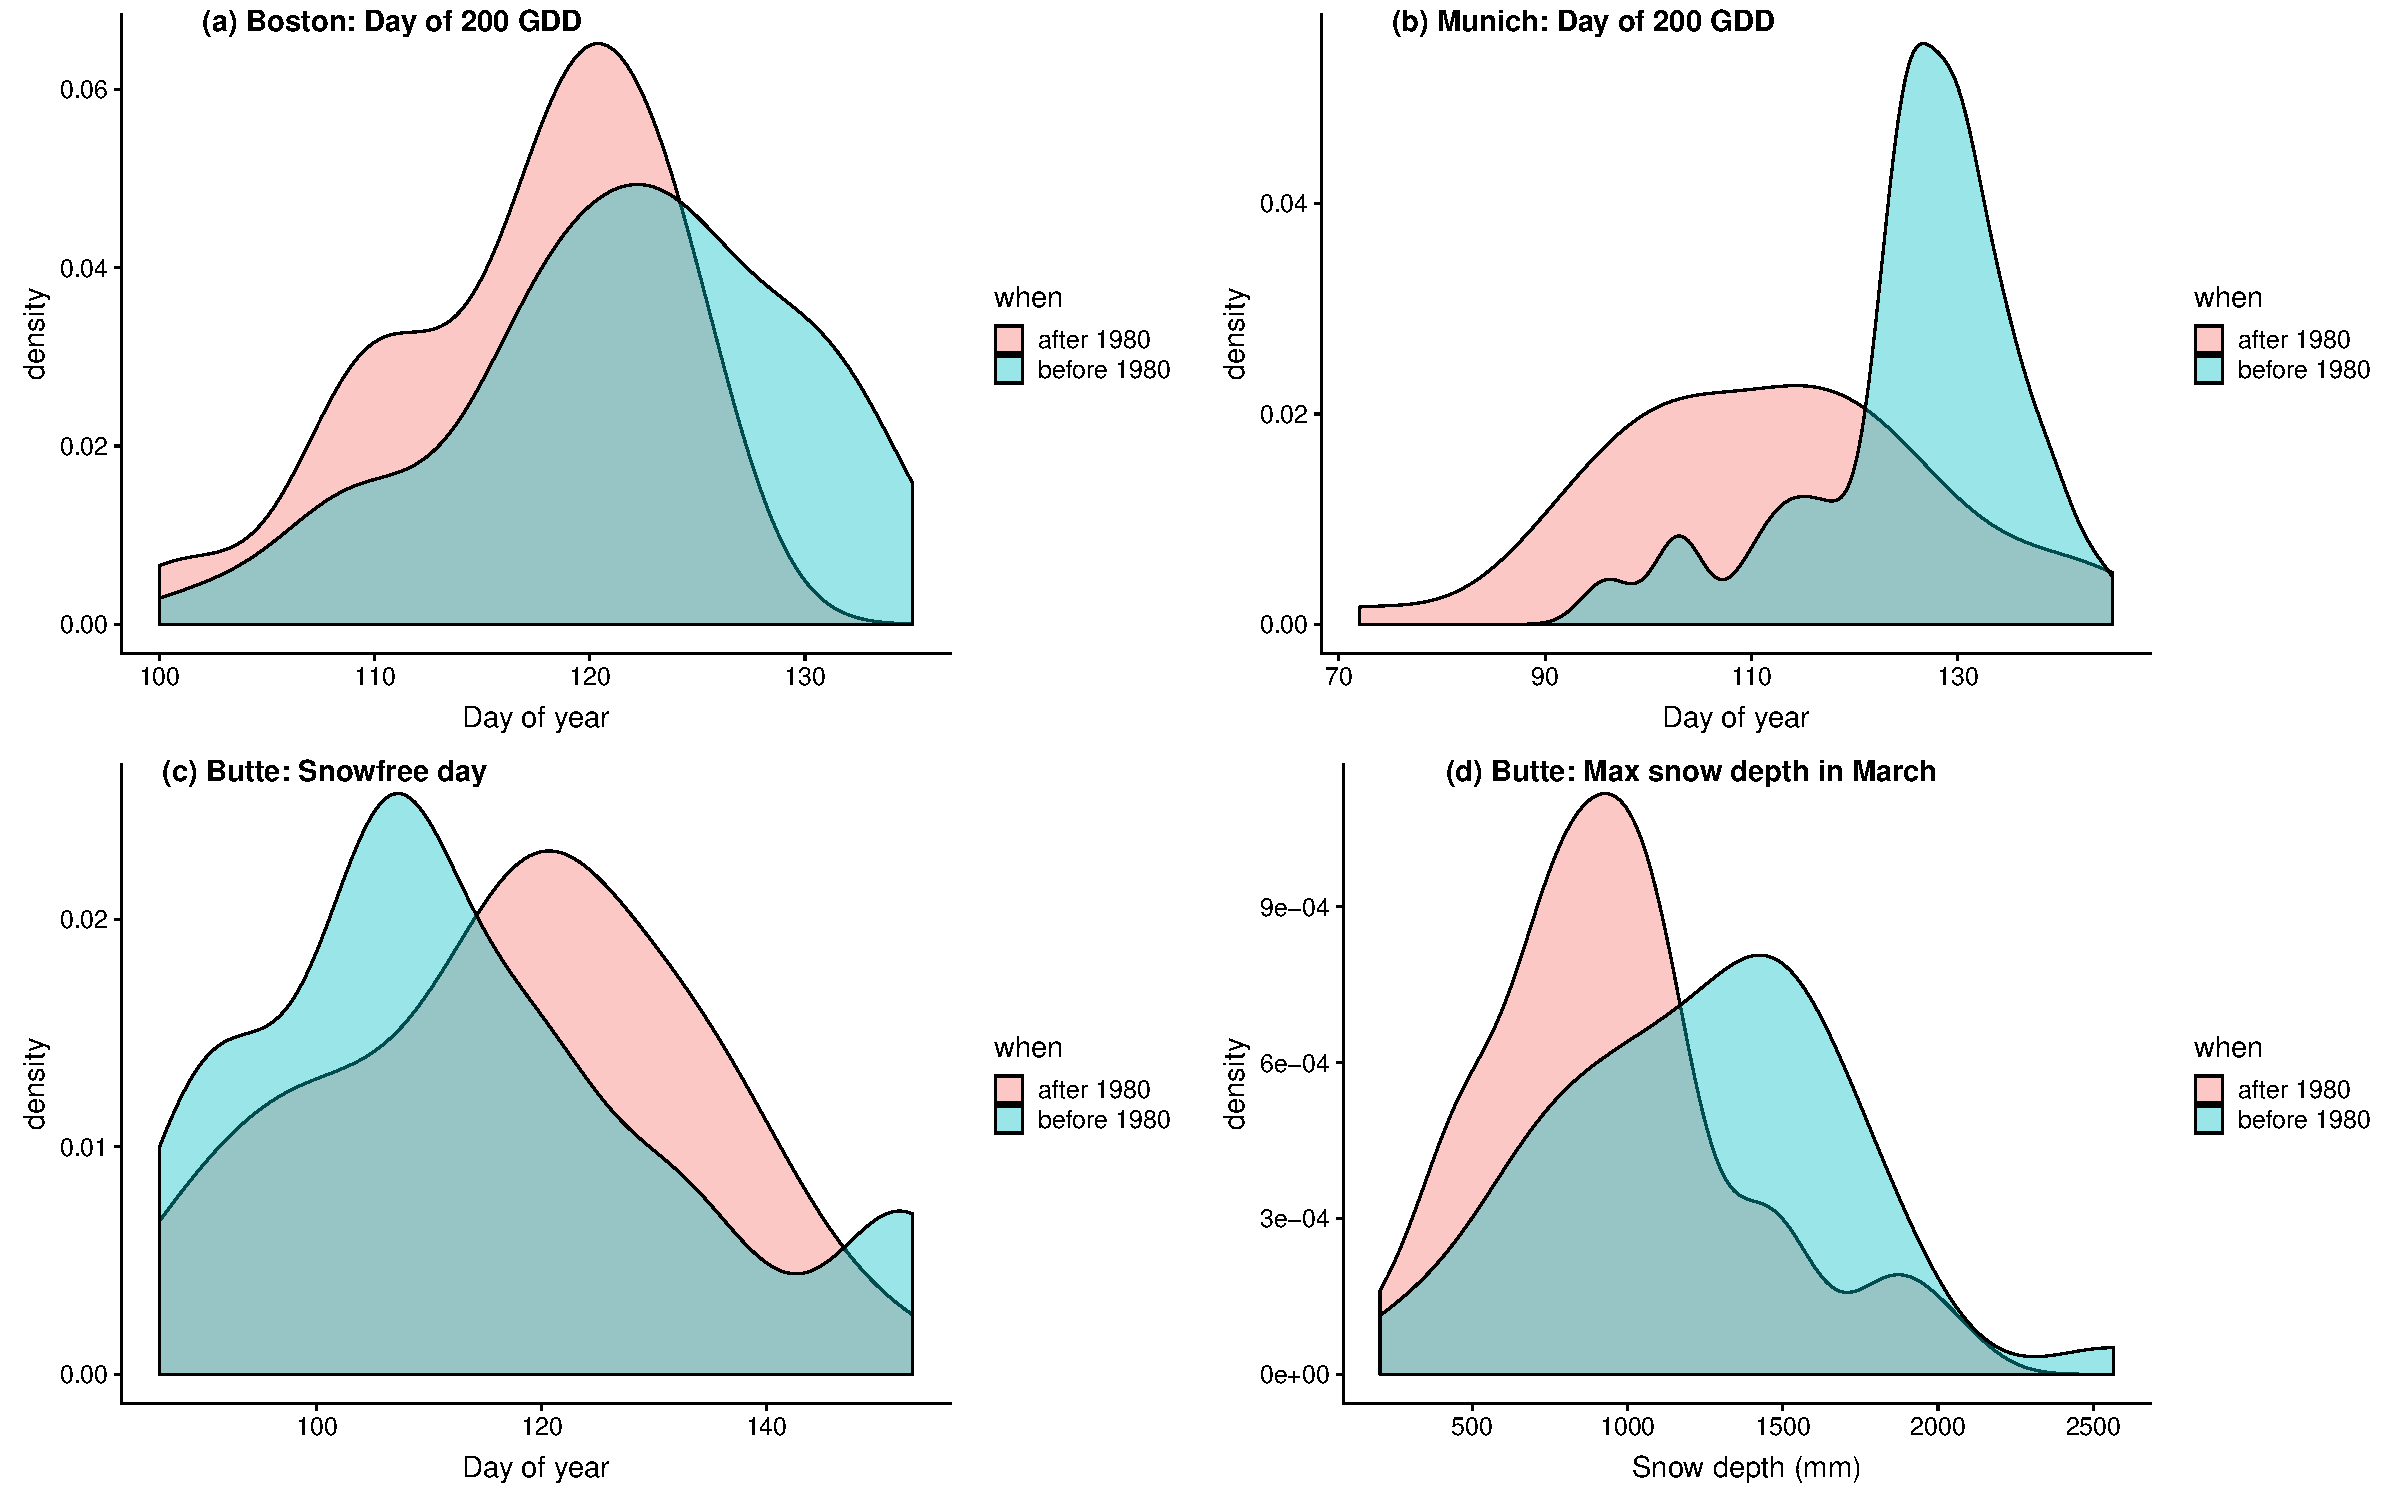
\includegraphics[width=1\textwidth]{..//..//..//R/graphs/otherdat/climdata.pdf}
\caption{Boom, we define ET.} 
 \label{fig:defineET}
\end{figure}

\begin{figure}[h!]
\centering
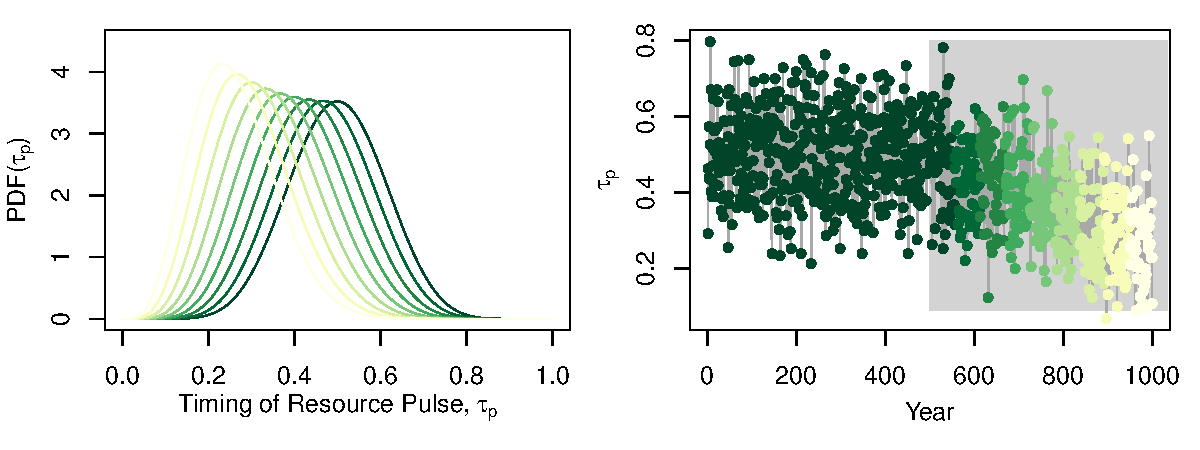
\includegraphics[width=1\textwidth]{..//..//..//R/graphs/modelruns/manuscript/modelsuppAlt.pdf}
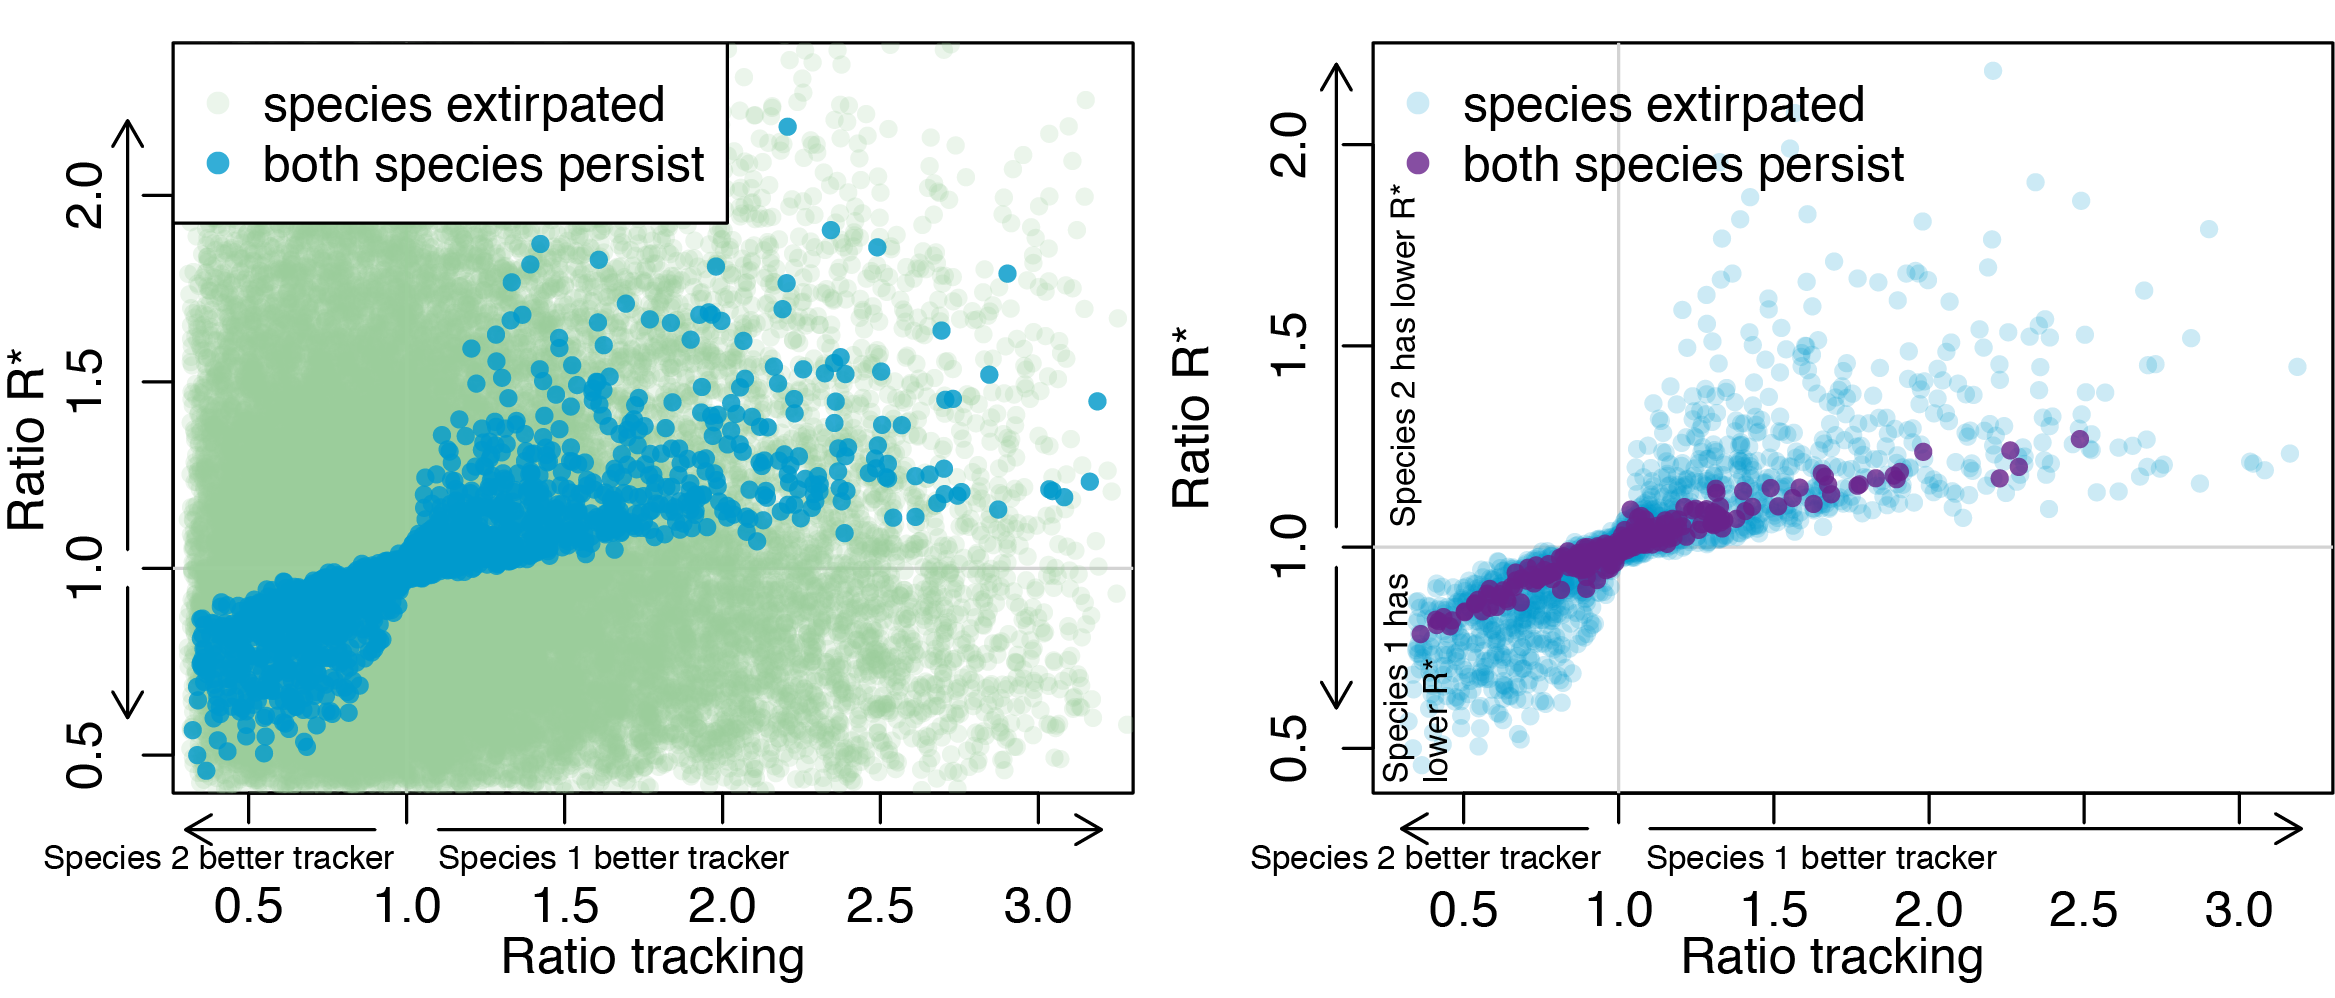
\includegraphics[width=0.96\textwidth]{..//..//..//R/graphs/modelruns/manuscript/alpharstar_2panelwide_adj.png}
\caption{Example of how non-stationarity can reshape communities in a simple model. We shifted the environment (top panels) by changing the timing of the resource pulse from a stationary period ($\tau_{p} \sim \beta(10,10)$ for the 500 years) to a nonstationary period ($\tau_{p}\sim \beta(5,15)$ over the 500 years), then examined outcomes for two-species communities (bottom panels) where tracking (X axis: species 1/species 2) trades off with $R^*$ (Y axis: species 1/species 2): each point represents one two-species community color-coded by whether both species persisted or one or more species was extirpated through 500 years of a stationary environment (bottom-left), followed by an additional 500 years of non-stationary environment (bottom-right, only two-species communities that persisted through the stationary period are shown).}
\label{fig:modelfig} 
\end{figure}

\begin{figure}[h!]
\centering
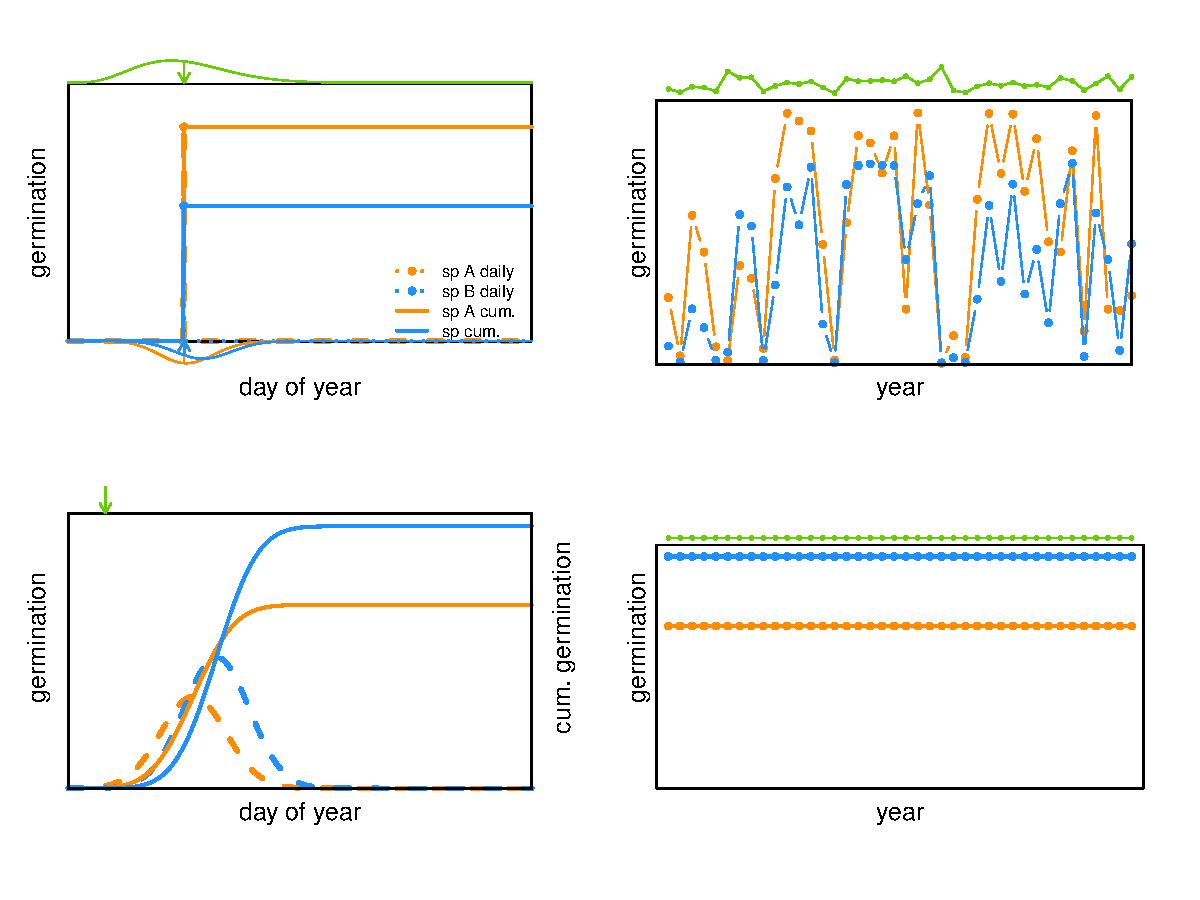
\includegraphics[width=1\textwidth]{..//..//..//R/graphs/conceptual/PriorityEff_BetHedge.pdf}
\caption{Tracking can be conceptualized as changes in priority effects or changes in storage effects.  In a priority effect model (A,B), the coexistence mechanism is a within-year tradeoff between, an early-germinating species that pre-empts resources (sp 1) and late-germinating species that is a superior resource competitor (sp 2) (A, where green arrow indicates the start of season); no between-year variation is required to maintain coexistence. In a storage effect model (C,D), variation in the timing of the start of season (indicated by the distribution in green, top of C) results results in differential species-response to the environment (illustrated by species-specific germination curves, bottom of C); this interannual variation in species-response to the environment (D) - along with a seedbank or other interannual storage mechanism - can maintain coexistence through reduced interspecific competition.}
\label{fig:conceptmodels} 
\end{figure}


%=======================================================================
% References
%=======================================================================
\clearpage
\newpage
\bibliography{/Users/Lizzie/Documents/git/bibtex/LizzieMainMinimal}
\bibliographystyle{/Users/Lizzie/Documents/git/bibtex/styles/ecolett.bst}


%=======================================================================
% Tables
%=======================================================================

%\begin{center}  
%\begin{table}
%\caption{Key differences between PWR and traditional PCMs such as PGLS.}
%\begin{tabular}{ | p{4cm} | p{5.5 cm} | p{5.5 cm} |}   \hline 
%& PWR & PCMs (e.g., PGLS) \\ \hline \hline
%Major goal & Study of evolution of correlation between variables across species & Study of evolution of correlation between variables across species\\ \hline
%\emph{Assumption 1:} Nature of correlation between two or more variables & Non-stationary (changes through phylogeny in a phylogenetically conserved fashion) & Stationary (constant) throughout phylogeny (all variation is noise) \\ \hline
%\emph{Assumption 2:} Completeness of variables & Substitutes phylogeny for variables (simple or complex) not in the model that interact with variables in the model & Assumes variables in model are primary drivers of correlational relationship \\ \hline
%Inferential mode & Usually exploratory & Hypothesis testing (statistical significance)\\ \hline
%Outputs & Coefficients of regression changing through the phylogeny & p-value and single set of coefficients presumed to apply to entire phylogeny with their confidence intervals\\ \hline

%Method to avoid overfitting & Cross-validation (boot-strapped determination of optimal band-width for accurate prediciton of hold-outs) & Exact analytical model of errors and degrees of freedom\\ \hline \hline
%\end{tabular}
%\end{table}
%\end{center}

%=======================================================================
% Paste in revision letter here to make line numbers work
%=======================================================================
\nolinenumbers


\end{document}
%%%%%%%%%%%%%%%%%%%%%%%%%%%%%%%%%%%%%%%%%%%%%%%%%%%%%%%%%%%%%%%%%%%%%%%%

\begin{enumerate}
\item Figure for ... The shape of this underlying distribution varies across systems and in how it is measured---the amount of rainfall in semi-arid systems is often highly skewed compared the thermal sum of many temperate growing season
\item With climate change, warming has increased mean temperatures over time, with minimum temperatures generally increasing mre than maximum---this results in an underlying distribution for daily temperature where the mean is both increased through time and the variance is decreasing (Munich garden? Maybe add San Dieg precip example?
\item Real-world data showing stat/non-stationarity in environment (ideally $\tau_{p}$) 
\item Real-world data showing tracking (and less tracking)
\item $\tau_{i}$ vs. R* trade-off and histogram of persisting $\tau_i$ under stat/nonstat $\tau_{p}$ environment
\item alpha vs.$\tau_i$ trade-off and histogram of persisting alpha under stat/nonstat $\tau_{p}$ environment
\item alpha vs. R* trade-off and histogram of persisting alpha under stat/nonstat $\tau_{p}$ environment
\item (Scratch this one: we're pretty sure it required a crappy $\tau_i$ to survive the initial stationary period, then be favored in second time period and we're not so sure crappy $\tau_i$ species survive the initial stationary period) time-series of one run showing years where $\tau_i$ of one species is close to $\tau_{p}$ and other years where $\tau_i$ of other species is close to $\tau_{p}$ (and show this shift under nonstat)
\item non-stationarity in $R0$ and $\tau_{p}$
\end{enumerate}


%=======================================================================
% to-do listing
%=======================================================================

\listoftodos

%=======================================================================
\section*{Other loose ends}
%=======================================================================

% Old hypothesis: Without tracking we may predict benefits to early-colonizers decline with earlier seasons. As start-date moves earlier, early folks lose benefit (assuming they tend to often go at optimum time) and you get more late folks. Late species may be less different than one another---and less responsive to environment. Early folks, effectively, become more similar to environment. 

% Environmental variability means many species should benefit from tracking their environment. We focus here on environmental tracking through time (often referred to below as `tracking') rather than through space because of its well-established links to individual-level physiology, yielding a more robust understanding of what environmental cues determine tracking \citep{chuineJTB,Chew:2012pd}, and because it has been repeatedly linked to performance and other fitness-related metrics. Temporal environmental cues, however, are often linked to species' ranges \citep{Morin:2008vp,arabid2011}, thus we expect much of this work could extend to environmental tracking through space. 
% Definition of tracking: correlation between a recurring biological event and something else in its environment

Many (or potentially all) species use abiotic cues to trigger major phenological events. These cues in turn result in different rates of tracking. At one extreme, some cues yield a fixed timing, resulting in no tracking over time. A common example of a fixed cue is photoperiod, which results in event timing that is constant across years (but variable across space, allowing---for example, later timings poleward for spring events) and appears widespread for some insect emergence and for fall senescence of many trees \citep{Denlinger2017,lechowiczbook2002}. Fixed timings are perhaps the simplest option and may be efficient for events where there is low predictability, low variability, or low costs to being too late or early. In cases where there is a high cost to mis-timing an event across a variable environment, cues that yield more variability in timing are far more prevalent and usually rely on climate. Temperature is a widespread cue for start of season events with many organisms needing a certain thermal sum to start visible growth. Such a cue has the benefit of shifting the date of an event early or late, depending on climatic conditions, each year, but may be a poor cue in years with aberrant events (e.g., a late frost). In most systems, species must use environmental cues such as temperature to forecast the ideal date for an event---a date which is only obvious in retrospect. ...  Measuring tracking depends on many factors (see Box `What underlies variability in species tracking?'). 






